\chapter{Test and Validation of the Proposed Solution }

\renewcommand{\chaptername}{Chapter}

\section*{Introduction}
After the development conducted in the previous chapter, the results of the implementation 
and concrete tests are highlighted and discussed.
This part outlines:

* the initial conditions of the test: Coordiantes of the robot, and the coordinates of the station 
and its configuration and constraints. and the test scenarios.
* the results of path planning of the pattern path. 
* results of the evaluation approach 
* results of the path optimization
* Analysis of the Metaheuristics
* Comparison to OMPL
* the robot following the generated path. Screenshots of the robot at 3 intermediate positions and mention 
the coordinates. the robot in its final position.

Fot this section 3 test environments are used:
\begin{itemize}
    \item Independant Simulation Environment: This environment is created outside of the RACK 
    environment to validate the chosen approaches before implementing the developed features 
    on the real system. It recreates the Station and the Shelf without sensor inputs or kinematic constraints.
    To simplify the test, the robot is modeled by a point instead of its proportional chassis size.

    \item RACK simulation environment: It is the simulation environment used in the team to simulate 
    the outcomes of the developed features in the same conditions as the real test. It includes all the sensor 
    input and makes it available for the test: Localization, Obstacle Detection, and Object Recognition features.
    It can be Offline or Online
    \begin{itemize}
        \item Offline Testing: is the re-creation of the warehouse and the test environment in a complete model
        as seen on figure \Ref{warehouse}. A simulated robot is available to place at a starting point, 
        to navigate the planned paths as well
        as to perceive its surroundings and use the sensor input for it processings. Objects like simulated 
        obstacles can be added. 
        \item Online Testing: is a projection of the test on the AMR to the Simulation environment.
        The simulation visualizes the output of the sensors like scan points and makes a debugging 
        tool available for interpretation of results, debugging, and optimization.
    \end{itemize}

    \item AMR tests: the AMR is commissioned with the test algorithms, validated through the RACK simulation
    environment tests. The truck navigates the planned paths in the real warehouse and deals with real stations, 
    shelves, pallets, obstacles and general surrounding objects.
\end{itemize}

\section{Path Creation Test Results and Validation}
The implemented Path Creation Approach explained in section 3.2.3 was first tested in a simulation environment
composed of one Station. This environment emulates the RACK model of the test warehouse and was used to test 
and validate the approach before testing it inside the RACK simulation first and then on the AMR.

For this environment, the implementation results of the subpolygons from section 3.1 were used for the path creation.
The created subpolygons are used as transition zones. 
As a first test of pure path creation, the transition points are previously fixed at the center of the 
subpolygons. The path is created by placing the robot in the simulation in a starting position and testing 
different target locations.

The obtained results are of smooth splines adhering to the pattern and linking the truck to the destination pallet 
while passing by a transition location. 
The Independant Simulation Environment tests show the pattern spline-based path as given by figure \Ref{Test_clone}:
The path start at the truck's position, transitions in one of the transition subpolygons to change driving 
direction and joins the target. 
The resulting path on the RACK simulation environment which is the real testing environment show as well 
the creation and plotting of the pattern path on the simulated station as given by \Ref{driving} and \Ref{Test_Simu}.

This approach is validated and is ready as a basis for the next test steps. 
The validation is for the following reasons:
\begin{itemize}
    \item The path creation module integrates the subpoygon functionality successfully: the use of a transition
    point from the subpolygons is effective when tested with a complete path.
    \item The created paths satisfy the intended pattern: they link the truck to the transition point, then, 
    the latter to the target. Inside the RACK simulation environment, it was verified that the direction 
    change occurs: the AMR switches from a negative speed at the first section when driving in opposite 
    direction the first part of the spline path until the transition point, to a positive speed when driving in 
    main driving direction the second part of the spline path from the transition point to the target.
    \item The paths link the start to the chosen target accurately which reflects the validation of the 
    transformations implemented at the development section of the Path Creation.
\end{itemize}

\begin{figure}[H]
    \centering
    \begin{minipage}{0.45\textwidth}
        \centering
        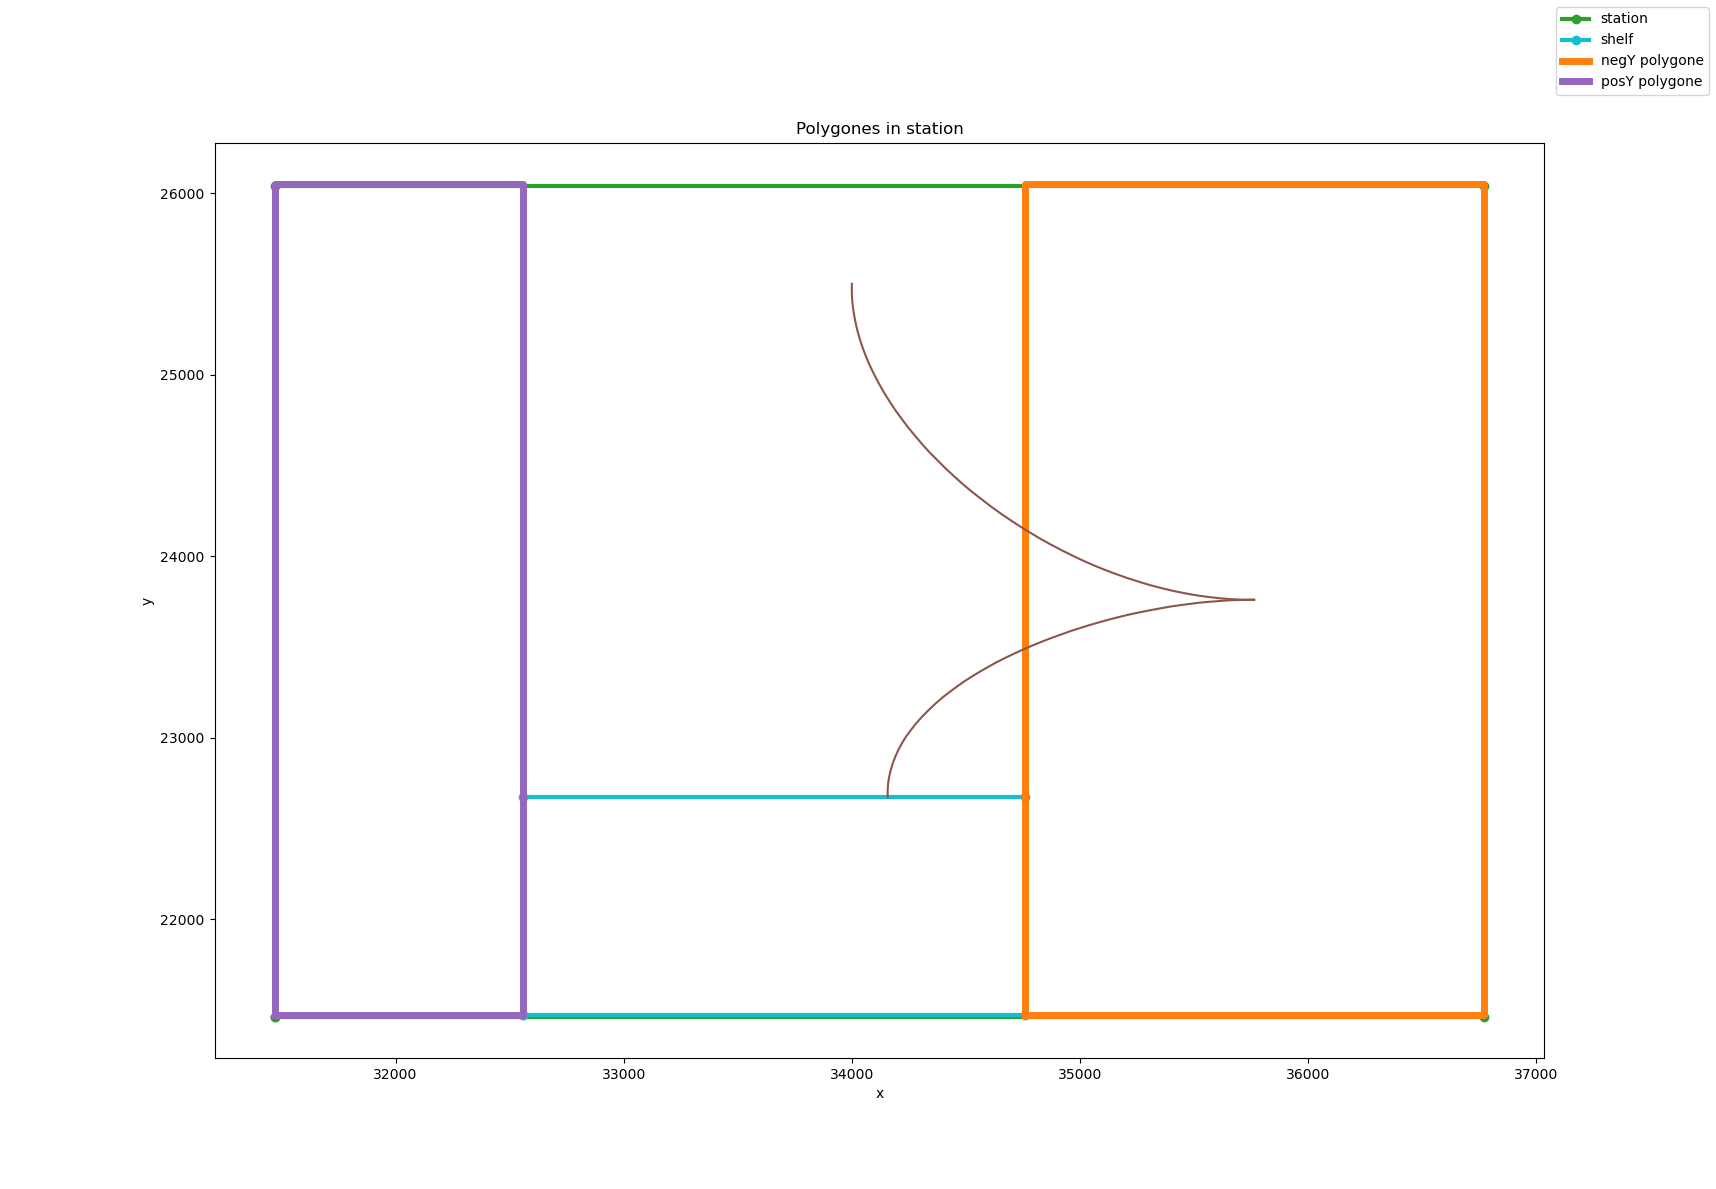
\includegraphics[width=3in]{images/Chap2/spline_split.png} 
    \end{minipage}
    \begin{minipage}{0.45\textwidth}
        \centering
        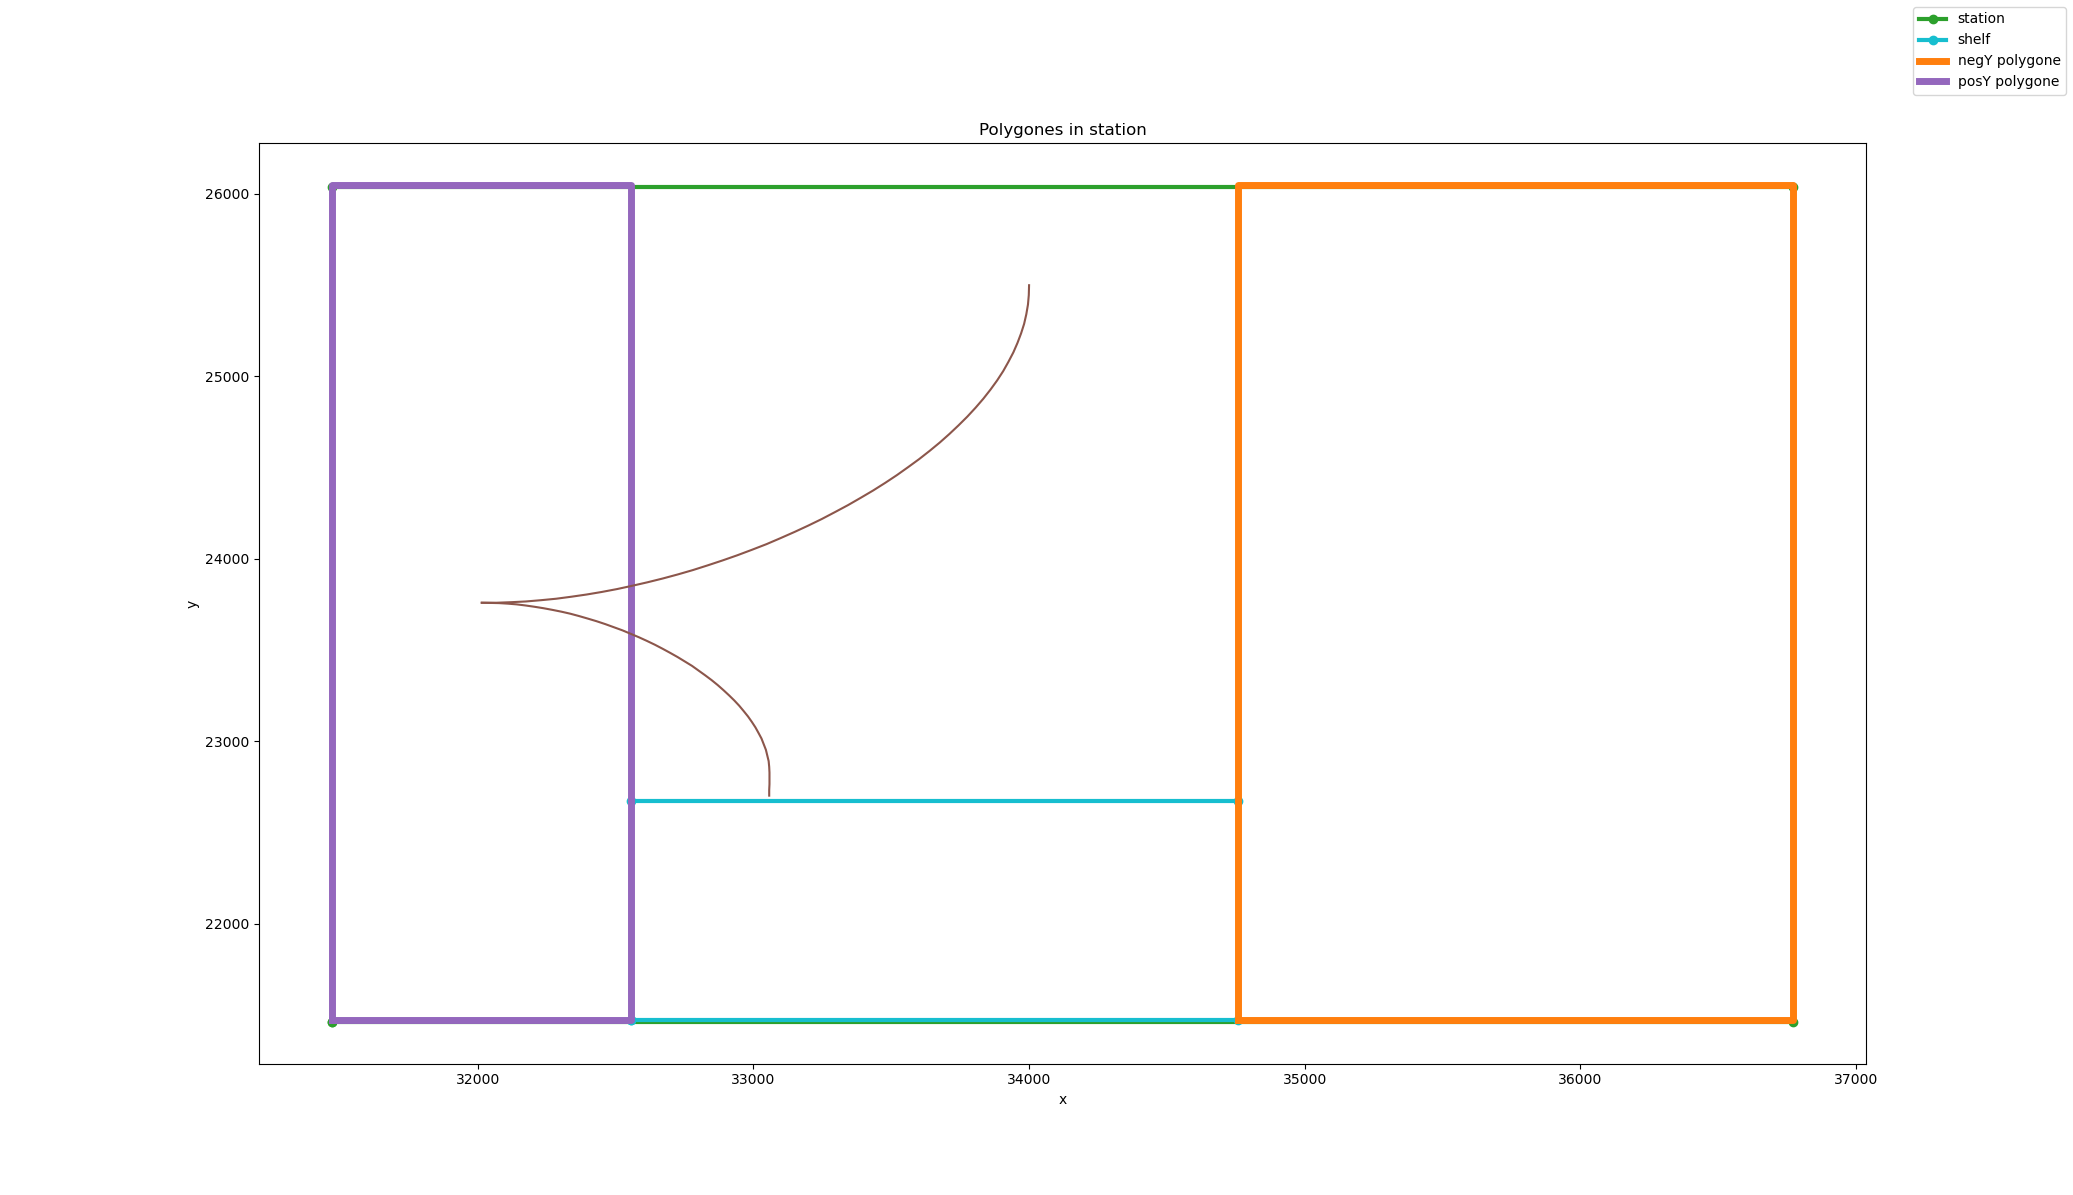
\includegraphics[width=3.5in]{images/Chap2/spline_split_posY.png}
    \end{minipage}
    \caption{Test Results on Cloned Test Environment}
    \label{Test_clone}
\end{figure}

\begin{figure}[H]
    \begin{center}
        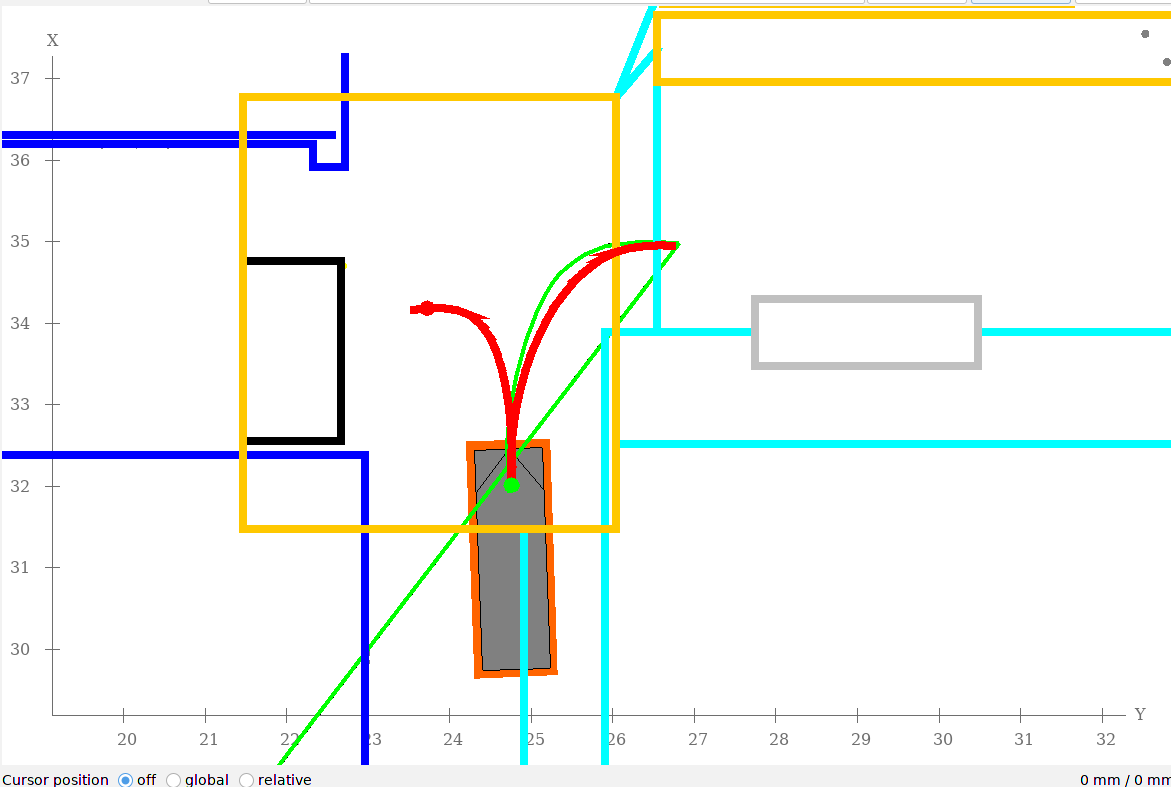
\includegraphics[width=4in]{images/Chap2/Pattern_spline_simulation_3_driving.png}\\
        \caption{Test Results on the Simulated Environment: Truck driving the Spline-based Pattern path}
        \label{driving}
        \end{center}    
\end{figure}

\begin{figure}[H]
    \centering
    \begin{minipage}{0.45\textwidth}
        \centering
        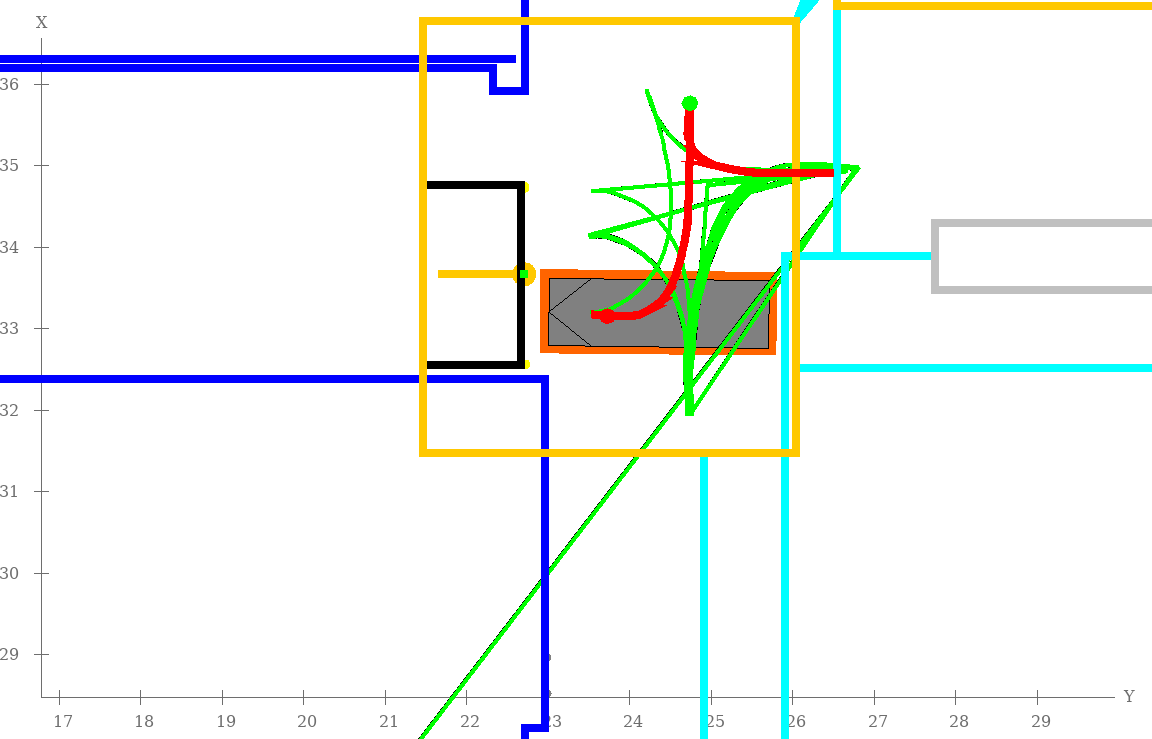
\includegraphics[width=\linewidth]{images/Chap2/Pattern_spline_simulation_1.png} % Replace with your figure
    \end{minipage}
    \begin{minipage}{0.45\textwidth}
        \centering
        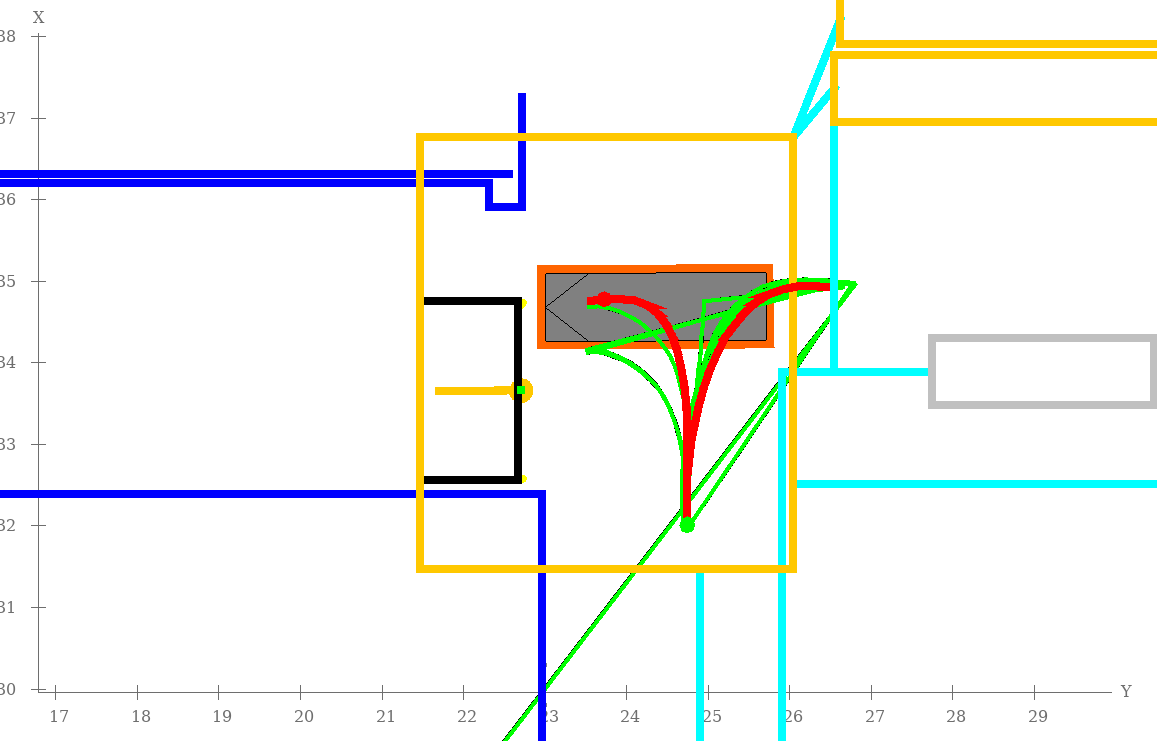
\includegraphics[width=\linewidth]{images/Chap2/Pattern_spline_simulation_2.png} % Replace with your figure
    \end{minipage}
    \caption{Test Results on the Simulated Environment: Truck at the Destination}
    \label{Test_Simu}
\end{figure}



\section{Path Evaluation Test Results and Validation}
In order to discriminate the Path Evaluation methods,
both approaches (3.3.2.1 and 3.3.2.2) were tested in the Independant Simulation Environment. 
Tests were ran on 10 different spline paths  that were generated with transition points scattered in 
the station \Ref{Mult_splines}.
Different locations of transition points were used to stress the metric outcomes by creating good and bad paths. 
The Exponential Weighted Path Evaluation was tested with \(\alpha\) = \(2\), \(\beta\) = \(0.0007\), 
\(\omega_c\)= \(0.7\) and \(\omega_L\)=\(0.3\).
The results are shown in figure \Ref{Test_Eval_Exp}: The bar chart reflects the Evaluation score of each 
spline path from figure \Ref{Mult_splines}. Each bar color reflects the same color spline.
The Normalized Weighted Path Evaluation was ran for two tests on the same splines set with 
\(\omega_c\)= \(0.7\) and \(\omega_L\)=\(0.3\) as well as 
\(\omega_c\)= \(0.5\) and \(\omega_L\)=\(0.5\). 
The results are shown in figures \Ref{Test_Eval_Norm1} and \Ref{Test_Eval_Norm2}
%comment on results:

For the Exponential Weighted Path Evaluation, the results are correct. It is easy to differentiate poor-quality paths. 
For example, the Blue spline was used as the reference path, while the Orange, Gray, and Purple paths were intentionally 
created as bad paths. The Orange and Gray paths generate significant curvature near the destination, making it 
challenging for the vehicle to navigate and arrive in the correct position and orientation given the narrow aisle 
that it has to turn and navigate in as shown by figure  \Ref{curv_problem}. Given the high curvature and the proximity to the
destination, the truck decelerates and moves very slowly. Changes that it stops at the correct orientation 
that allows it to pickup the pallet are very low. Such path have to be avoided at all costs. The Purple path is longer 
and curved at the starting area. Furthermore, the Brown path demonstrates the best overall fitness. Although it is 
short, it introduces high curvatures at the transition and destination areas. Compared to the Blue and Red paths, 
the Brown path is shorter but less smooth. 
The Exponential Evaluation also favors the Dark Green path to the Pink one, even though the concentrated 
curvature at the end of the green path is high.
In conclusion, this evaluation method is very sensitive to path length and less 
sensitive to high concentrated curvatures. This is due to the high factor of the length term, in the range 
of thousands of millimeters, and the low factor of the curvature term which is around the magnitude of \(10^{-3}\).
It is inconvenient to change the factors \(\omega_c\) and \(\omega_L\) by increasing \(\omega_c\) and 
decreasing \(\omega_L\) as the difference becomes huge while it is mandatory to attribute 
importance to both factors. Besides, this Metric is very sensitive to the change of the \(\alpha\) and \(\beta\) factors.
These factors must be carefully tuned to fit all use cases and account for varying station sizes and configurations. 
However, finding factors that are scalable across different use cases is not straightforward.

\noindent On the other hand, The Normalized Weighted Path Evaluation, chose the Red path as the best fitness, 
outperforming the Blue pattern path. This is due to the remarkable less curvature of the Red path at the start 
and transition locations due to its proximity to the transition polygon and distance to the destination.
These factors allow for smooth driving along the path.
Comparing figures \Ref{Test_Eval_Norm1} and \Ref{Test_Eval_Norm2}, the approach of outweighing the curvature 
over the length outperforms the equal weights approach. The Pink path is visibly better than the Brown due 
to better smoothness and the first weights approach discriminates them better. 
Given the challenges associated with driving along smooth paths, it is a strategic decision to prioritize the 
curvature term over the length term. Navigating a slightly longer path is far less difficult than handling a path 
with sharp curves.
This approach is not affected by the difference of range between length and curvature metrics given that 
they are each divided respectively by the reference path's length and curvature. This not only balances out the 
two terms but also makes it fit all use cases and account for varying station sizes and configurations given that 
the reference path is always relevnat to the present station.

As a final point, \textbf{the selected approach is the Normalized Weighted Path Evaluation} with \(\omega_c\)= \(0.7\) 
and \(\omega_L\)=\(0.3\) given by equation \Ref{Norm_function}.

The Path Evaluation Approach is validated and can be used for the path Optimization phase.
The approach was validated for the following reasons: 
\begin{itemize}
    \item The Selected Evaluation method satisfies the goal of optimizing path length and thus travel time
    and limiting high curvature and challenging turns of the bulky truck by optimizing curvature change.
    \item Using the Evaluation Method, good and poor quality pattern paths can be discriminated by 
    affecting a score to each path according to its properties and comparing them.
\end{itemize}

The approach is ready to be used as the cost function of the optimizer.

\begin{figure}[H]
    \begin{center}
        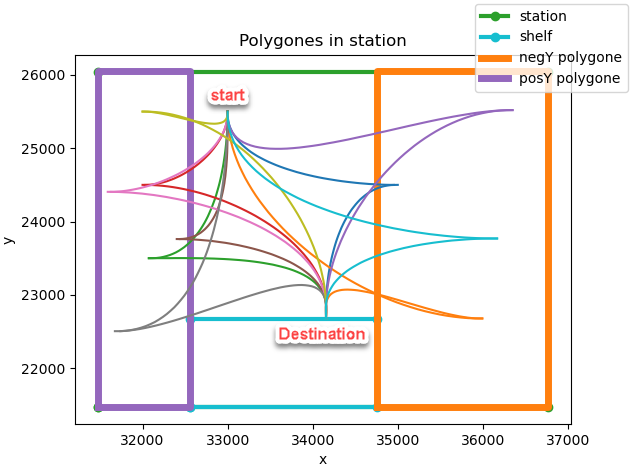
\includegraphics[width=4in]{images/Chap2/Mult_Splines_noted.png} % Replace with your figure
        \caption{Test Results on the Simulated Environment: Multiple Splines Visualization}
        \label{Mult_splines}
        \end{center}    
\end{figure}

\begin{figure}[H]
    \begin{center}
        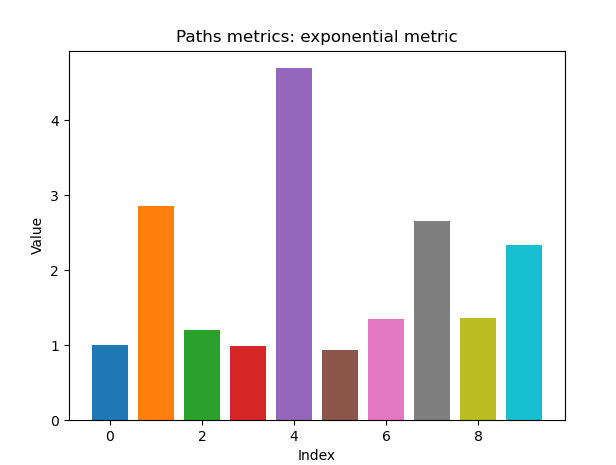
\includegraphics[width=4in]{images/Chap2/Exp_Results.png} % Replace with your figure
        \caption{Test Results on the Simulated Environment: Evaluation results of the Exponential Approach}
        \label{Test_Eval_Exp}
        \end{center}    
\end{figure}

\begin{figure}[H]
    \begin{center}
        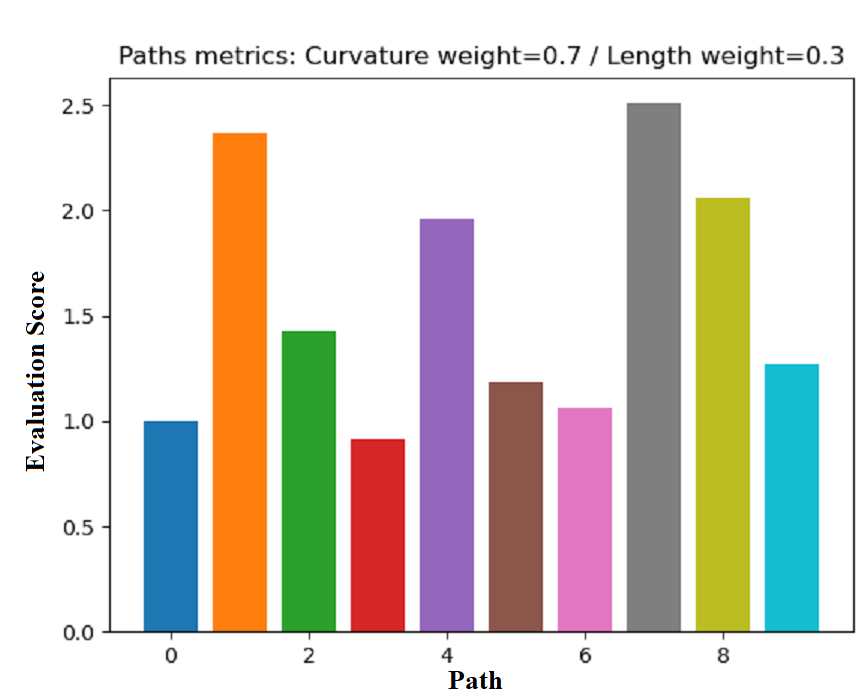
\includegraphics[width=4in]{images/Chap2/w_0.7.png} % Replace with your figure
        \caption{Test Results on the Simulated Environment: Evaluation results of the Normalized Approach
        with weighing out the curvature}
        \label{Test_Eval_Norm1}
        \end{center}    
\end{figure}
\begin{figure}[H]
    \begin{center}
        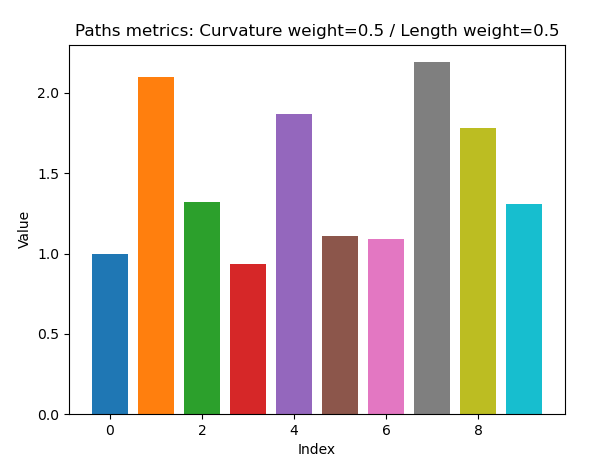
\includegraphics[width=4in]{images/Chap2/w_0.5.png} % Replace with your figure
        \caption{Test Results on the Simulated Environment: Evaluation results of the Normalized Approach
        with equal weights}
        \label{Test_Eval_Norm2}
        \end{center}    
\end{figure}

\begin{figure}[H]
    \begin{center}
        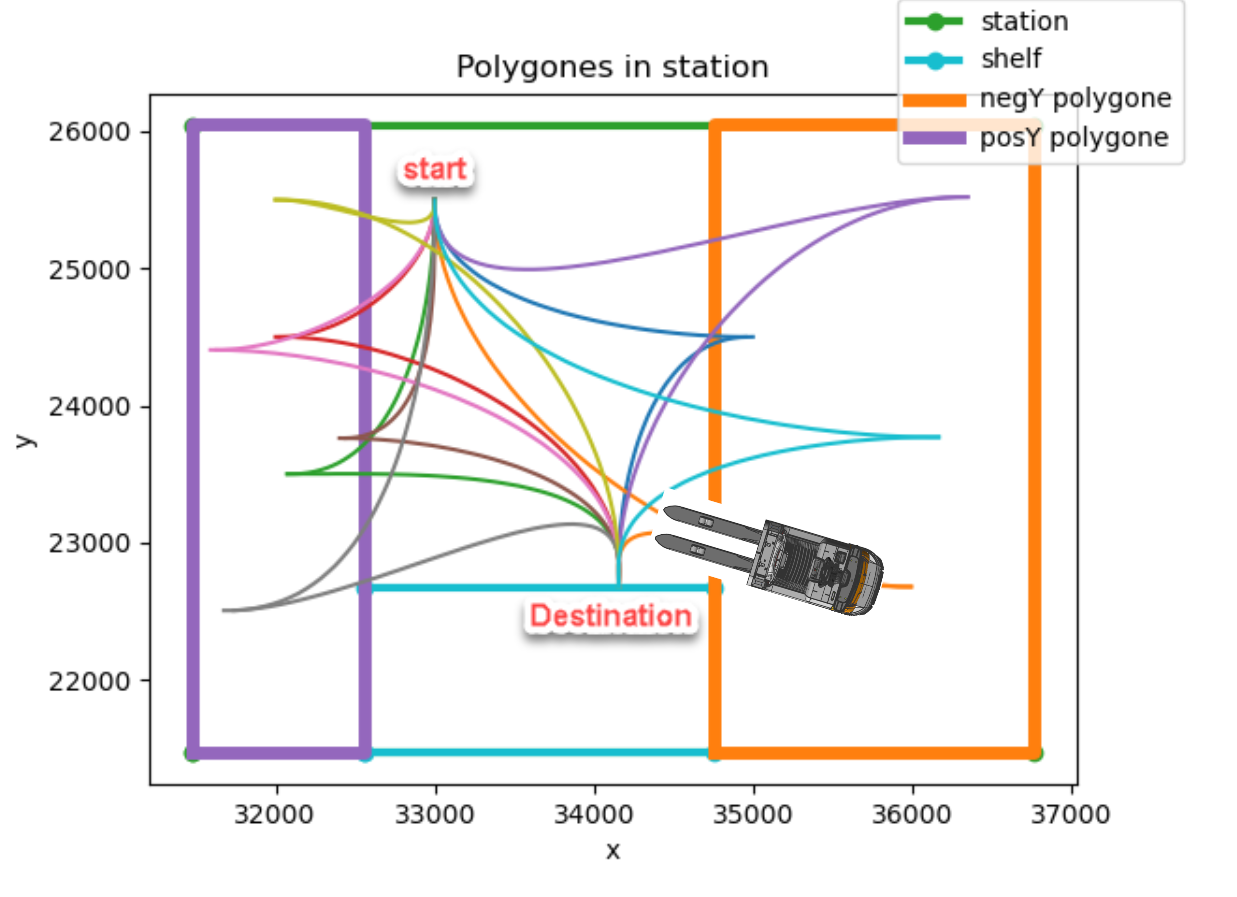
\includegraphics[width=4in]{images/Chap2/curv_problem.png} % Replace with your figure
        \caption{Navigating high curvatures in narrow areas}
        \label{curv_problem}
        \end{center}    
\end{figure}

\section{Path Optimization Test Results and Validation}

Using the Path Creation and the Selected Evaluation approach, the optimization approach is tested.
First the Optimizer is tested in an empty station, then it is tested against obstacles placed inside the station 
in different locations. 
The optimization algorithm is ran first on The 
Independant Simulation Environment to verify the relevance of the optimization approach to the pattern-based 
path. 
For this test, The Optimizer evaluates 10 generations of 10 paths for each subpolygon, it calculates the fitness value 
for each path and saves the overall best fitness value from both subpolygons. 
Figure \Ref{OptResult1} shows the result inside the Independant Simulation Environment for a station empty of obstacles:
The figure illustrates the candidate paths of the first of the 10 generations, along with the optimum paths from 
both subpolygons in bold Red and Brown "champion paths" as called in the algorithm. 
The algorithm successfully rejects poor quality paths like the lowest right red path which has two direction changes 
along the path due to the sharp turn in the beginning, and the highest left blue path that 
has an unfeasible sharp turn at the target.
The approach is validated at this stage. 

\begin{figure}[H]
    \begin{center}
        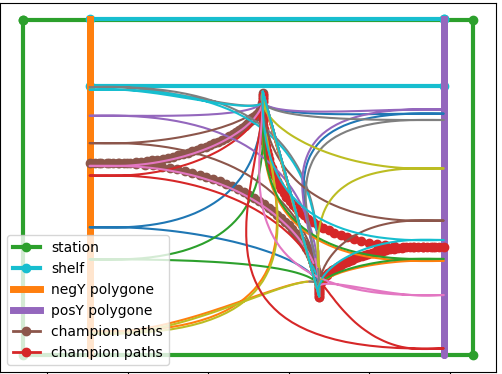
\includegraphics[width=4in]{images/Chap3/Gen1_crop.png} % Replace with your figure
        \caption{Optimizer results in empty station of one of 10 generations with the overall best paths 
        visualized in bold red and brown}
        \label{OptResult1}
        \end{center}    
\end{figure}


The second test is ran with obstacles placed in different positions in the station. 
The Algorithm results on figure \Ref{OptResult2} illustrate that the optimizer is capable of generating paths the avoid 
obstacles. The optimizer does generate paths that cross the quadrilateral obstacle but those paths 
are eliminated by better quality paths: the optimum paths in Brown. The quadrilateral obstacle was placed 
in a critical area, the center of the station to stress the optimizer. On the other hand, 
the rectangle obstacle was placed in the right corner of the station at a far distance from the start position,
the optimal transition area inside the subpolygon, and the target.
Although the two paths are  correct, the brown path is highly curved at the beginning because it avoids the 
quadrilateral obstacle. However, the red path is smoother at the start and destination segments of the path.

\begin{figure}[H]
    \begin{center}
        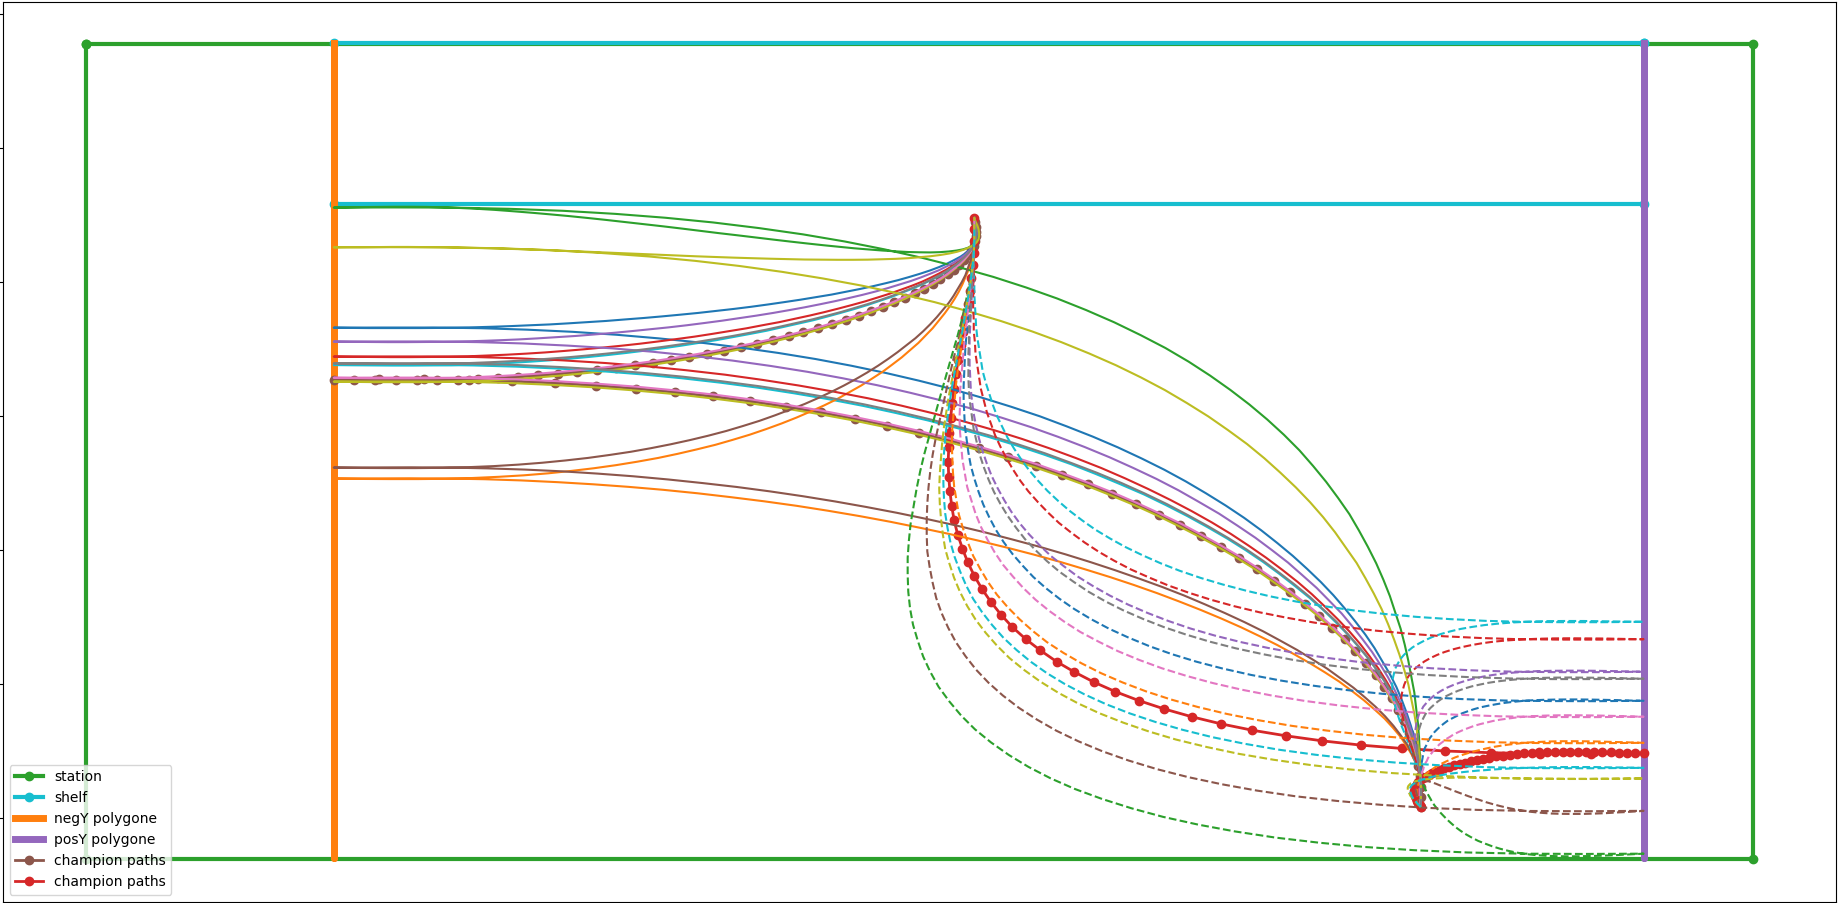
\includegraphics[width=4in]{images/Chap3/scenario3_crop.png} % Replace with your figure
        \caption{Optimizer results in presence of obstacles of one of 10 generations with the overall best paths 
        visualized in bold red and brown}
        \label{OptResult2}
        \end{center}    
\end{figure}

Another obstacle situation was tested and illustrated by figure \Ref{OptResult3}.
The obstacles in this situation were placed in the center of the station . 
For this case the regular optimizer was unable to find a solution that does not collide 
with the obstacles. However, by increasing the number of the waypoints (approach in section 3.4.2.1),
The optimizer was effective in finding collision free paths. 


\begin{figure}[H]
    \begin{center}
        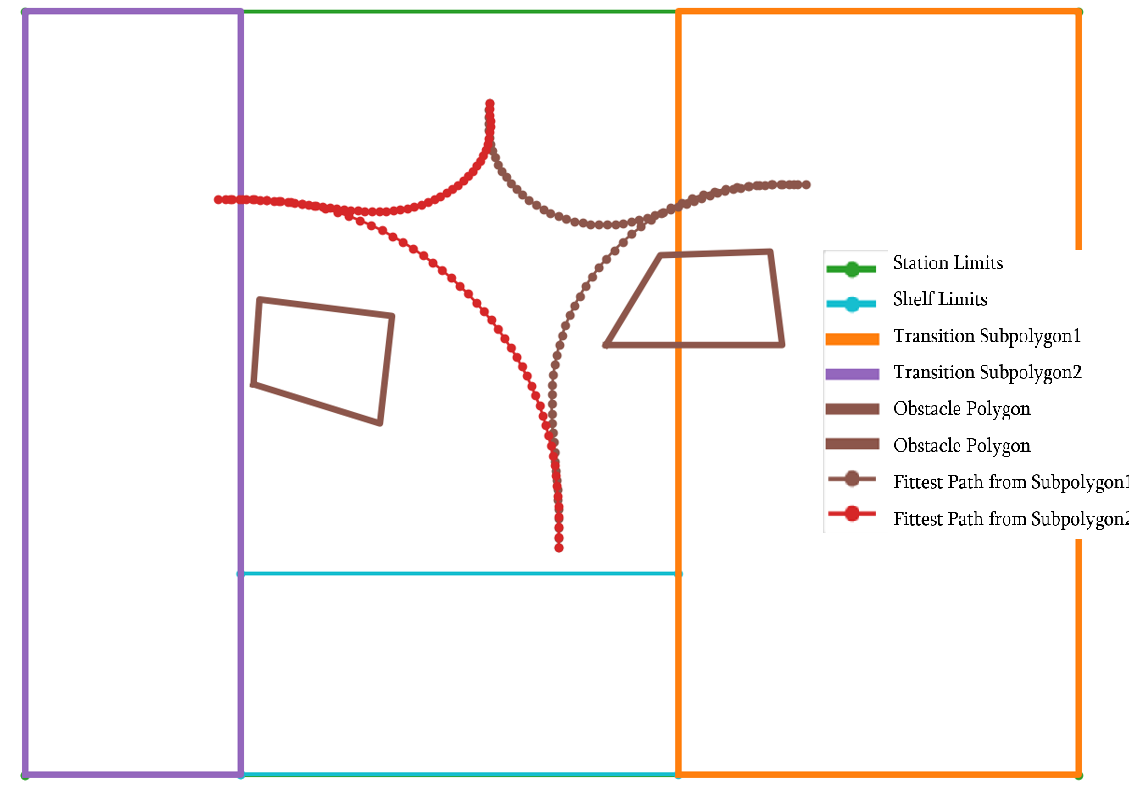
\includegraphics[width=4in]{images/Chap3/Figure_6.png} % Replace with your figure
        \caption{Optimizer results in presence of obstacles and influence of increasing path waypoints}
        \label{OptResult3}
        \end{center}    
\end{figure}

The approach is validated for a moderate complexity environment.

Given that the approach was validated in the Independant Simulation Environment, the tests are 
ran on the RACK Simulation Environment. Two test scenarios are created: 
The first is called the \(Simple Environment\) which is an obstacle-free station and the second is
called the \(Complicated Environment\) where an obstacle is placed in one side of the station. 
In reality, the \(Simple Environment\) is not simple because the sensors detect the warehouse walls,
shelves, objects, and other vehicles but the station area is free of stranger objects.
The test in the \(Simple Environment\) illustrated by figure \Ref{OptResult4} was done by placing the 
AMR in the simulation in the starting position (green rectangle) and selecting the target position on 
the simulation model. The expected target position is the red rectangle. 
The path is planned following the pattern and links the AMR from its start position to the target position.
The blue prints along the path represents the positions that the AMR will be at when driving the path.
It helps to make sure that the AMR will not collide with  

\begin{figure}[H]
    \begin{center}
        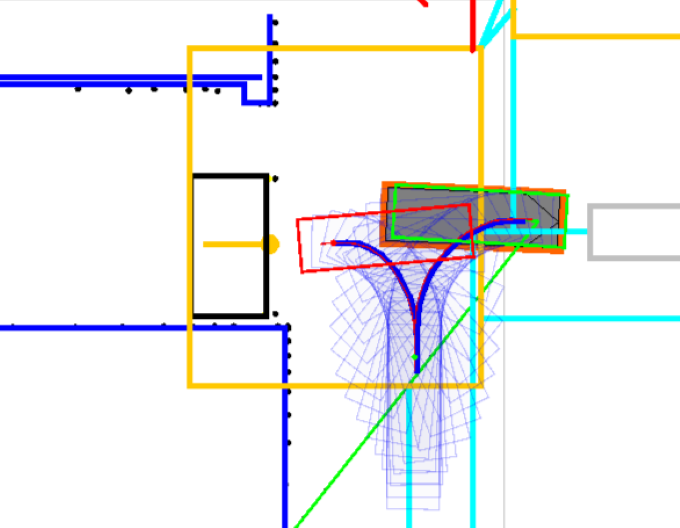
\includegraphics[width=4in]{images/Chap3/Start.png} % Replace with your figure
        \caption{Optimizer results in a simple environment tested inside the RACK simulation: Start Position}
        \label{OptResult4}
        \end{center}    
\end{figure}

\begin{figure}[H]
    \begin{center}
        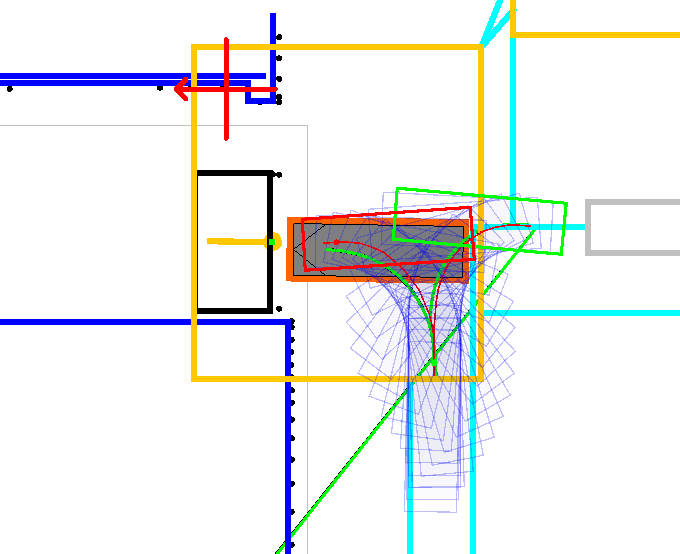
\includegraphics[width=4in]{images/Chap3/Target.png} % Replace with your figure
        \caption{Optimizer results in a simple environment tested inside the RACK simulation: Target Position}
        \label{OptResult5}
        \end{center}    
\end{figure}

\begin{table}[ht]
    \centering
    \resizebox{\textwidth}{!}{%
    \begin{tabular}{|p{3.5cm}|p{5cm}|p{5cm}|}
    \hline
    \textbf{Algorithm} & \textbf{Planning Time (Simple Environment) (ms)} & \textbf{Planning Time (Complicated Environment) (ms)} \\
    \hline
    Genetic Algorithm & 57 & 73 \\
    \hline
    PSO & 59 & 67 \\
    \hline
    ACO & 56 & 65 \\
    \hline
    Simulated Annealing & 80 & 78 \\
    \hline
    Differential Evolution & 27 & 44 \\
    \hline
    \end{tabular}%
    }
    \caption{Comparison of Planning Time for Different Algorithms in Simple and Complicated Environments (in milliseconds)}
\end{table}

\begin{table}[ht]
    \centering
    \resizebox{\textwidth}{!}{%
    \begin{tabular}{|p{4cm}|p{2.5cm}|p{2.5cm}|p{2.5cm}|p{2.5cm}|}
    \hline
    \multirow{2}{*}{\textbf{Algorithm}} & \multicolumn{2}{c|}{\textbf{Simple Environment}} & \multicolumn{2}{c|}{\textbf{Complicated Environment}} \\
    \cline{2-5}
     & \textbf{Negative Fitness} & \textbf{Positive Fitness} & \textbf{Negative Fitness} & \textbf{Positive Fitness} \\
    \hline
    Genetic Algorithm       & 0.549  & 0.32  & 31.0  & 0.449 \\
    \hline
    PSO                    & 0.561  & 0.349  & 1.159  & 0.38 \\
    \hline
    ACO                    & 0.542  & 0.384  & 50.0  & 0.417 \\
    \hline
    Simulated Annealing     & 0.45  & 0.394  & 1.258  & 0.428 \\
    \hline
    Differential Evolution  & 0.652  & 0.56  & 50.0  & 0,384 \\
    \hline
    \end{tabular}%
    }
    \caption{Comparison of Fitness Values of the optimum paths generated by Different Algorithms in Simple and Complicated Environments}
    \end{table}